\documentclass{standalone}
\usepackage{tikz}
\usetikzlibrary{patterns, positioning}
\usepackage[sfdefault]{ClearSans} %% option 'sfdefault' activates Clear Sans as the default text font
\usepackage[T1]{fontenc}

\begin{document}
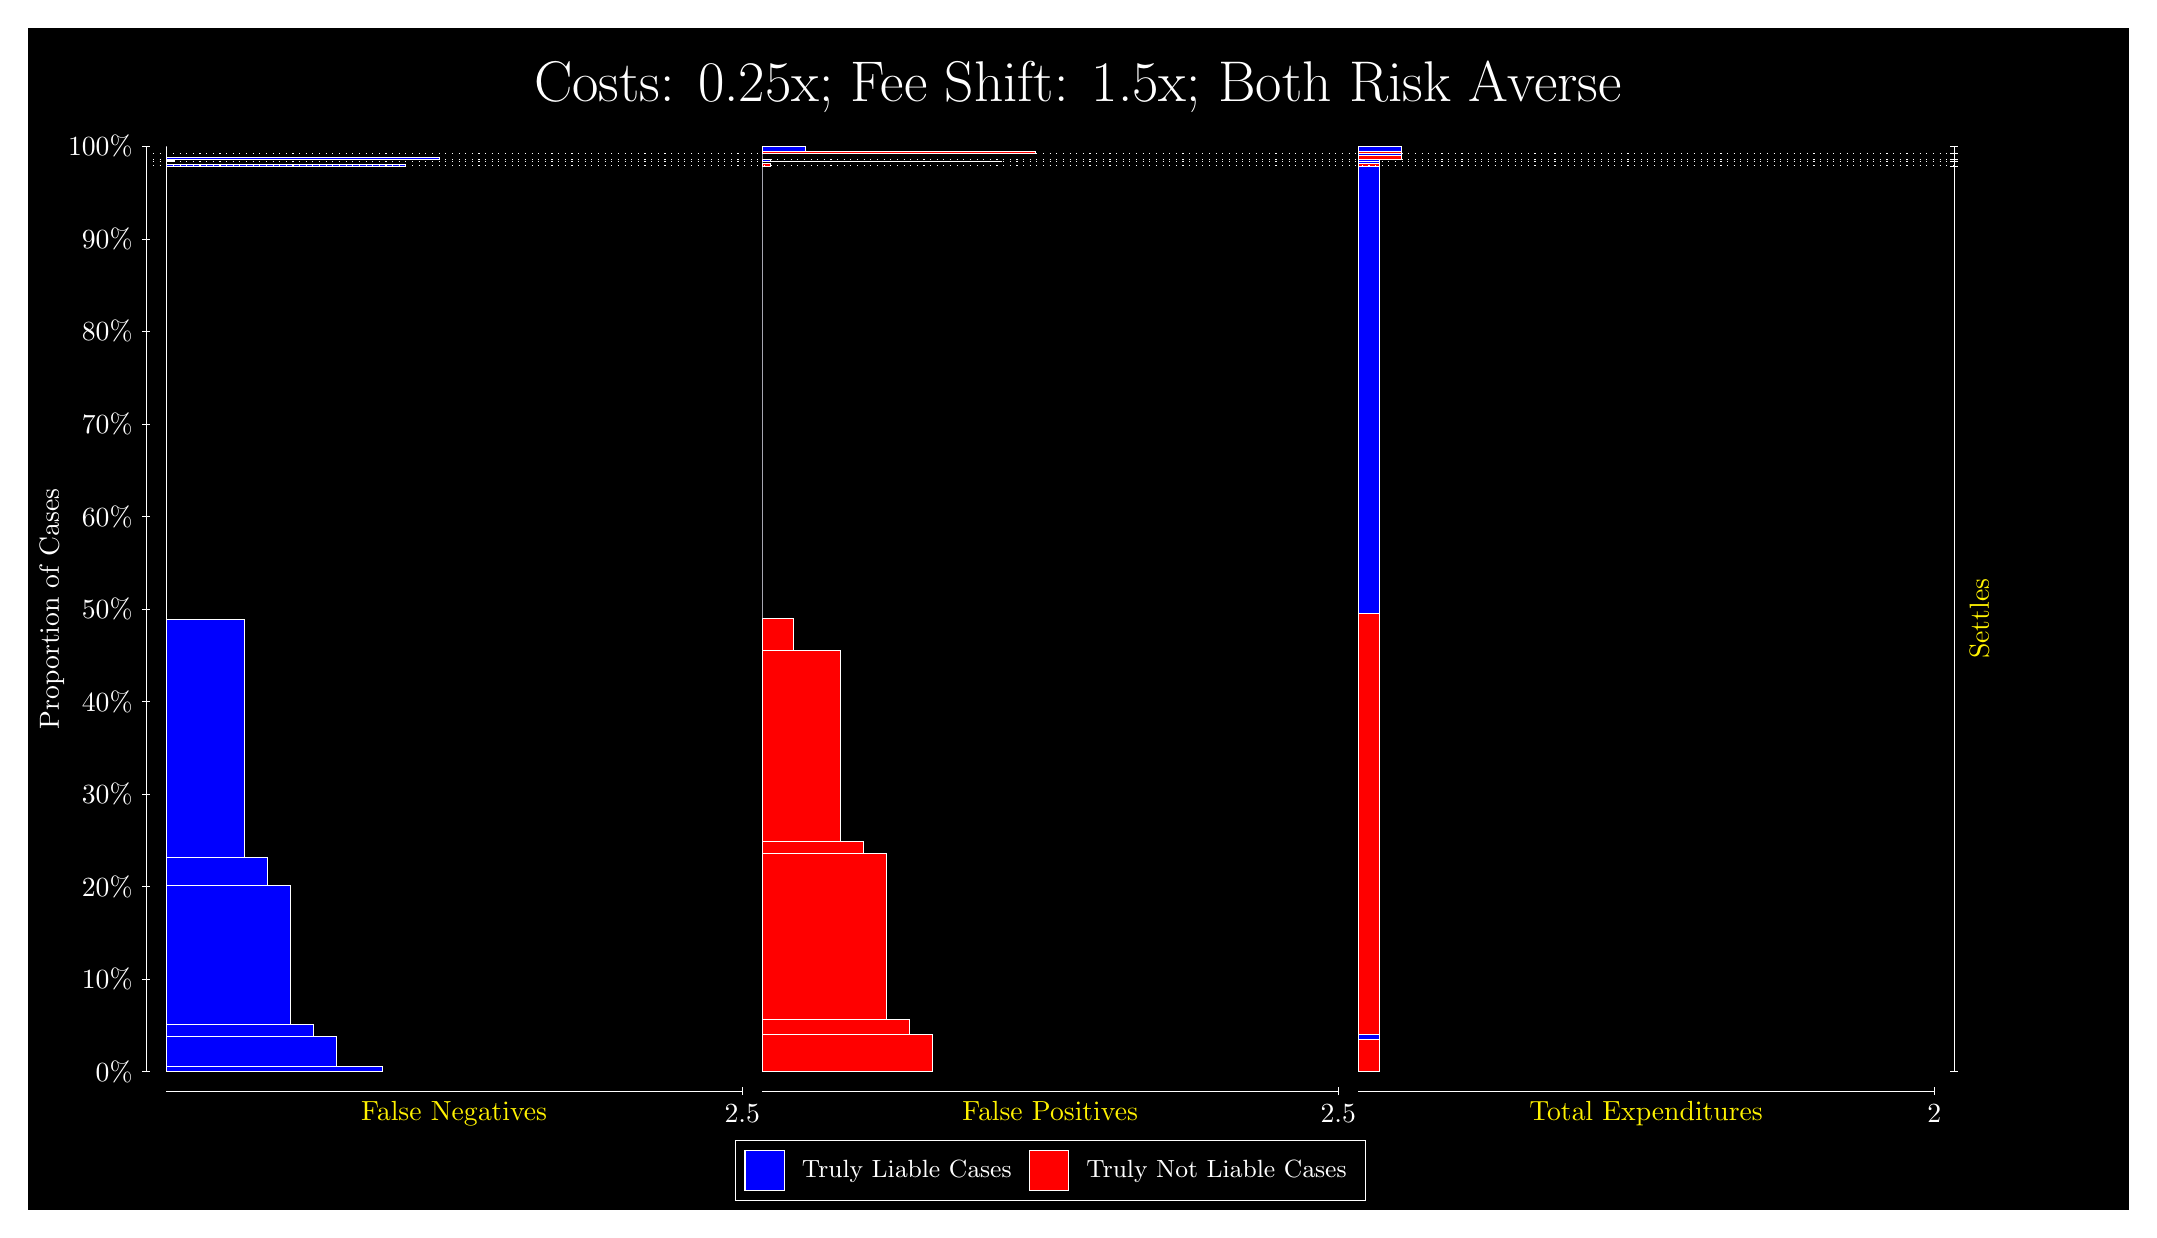
\begin{tikzpicture}
\draw[fill=black] (0,0) rectangle (26.667,15);
\draw[text=white] (0,13.5) rectangle (26.667,15) node[midway] {\huge Costs: 0.25x; Fee Shift: 1.5x; Both Risk Averse};
\draw[white, very thin] (1.5,1.75) -- (1.5,13.5);
\node[rotate=90, text=white, anchor=center] at (0.3, 7.625) {Proportion of Cases};
\draw[white, very thin] (1.45,1.75) -- (1.55,1.75);
\node[text=white, anchor=east] at (1.45, 1.75) {0\%};
\draw[white, very thin] (1.45,2.925) -- (1.55,2.925);
\node[text=white, anchor=east] at (1.45, 2.925) {10\%};
\draw[white, very thin] (1.45,4.1) -- (1.55,4.1);
\node[text=white, anchor=east] at (1.45, 4.1) {20\%};
\draw[white, very thin] (1.45,5.275) -- (1.55,5.275);
\node[text=white, anchor=east] at (1.45, 5.275) {30\%};
\draw[white, very thin] (1.45,6.45) -- (1.55,6.45);
\node[text=white, anchor=east] at (1.45, 6.45) {40\%};
\draw[white, very thin] (1.45,7.625) -- (1.55,7.625);
\node[text=white, anchor=east] at (1.45, 7.625) {50\%};
\draw[white, very thin] (1.45,8.8) -- (1.55,8.8);
\node[text=white, anchor=east] at (1.45, 8.8) {60\%};
\draw[white, very thin] (1.45,9.975) -- (1.55,9.975);
\node[text=white, anchor=east] at (1.45, 9.975) {70\%};
\draw[white, very thin] (1.45,11.15) -- (1.55,11.15);
\node[text=white, anchor=east] at (1.45, 11.15) {80\%};
\draw[white, very thin] (1.45,12.325) -- (1.55,12.325);
\node[text=white, anchor=east] at (1.45, 12.325) {90\%};
\draw[white, very thin] (1.45,13.5) -- (1.55,13.5);
\node[text=white, anchor=east] at (1.45, 13.5) {100\%};

\draw[white, very thin] (24.457,1.75) -- (24.457,13.5);
\draw[white, very thin] (24.407,1.75) -- (24.507,1.75);
\node[anchor=west] at (24.407, 1.75) {};
\draw[white, very thin] (24.407,13.252) -- (24.507,13.252);
\node[anchor=west] at (24.407, 13.252) {};
\draw[white, very thin] (24.407,13.306) -- (24.507,13.306);
\node[anchor=west] at (24.407, 13.306) {};
\draw[white, very thin] (24.407,13.331) -- (24.507,13.331);
\node[anchor=west] at (24.407, 13.331) {};
\draw[white, very thin] (24.407,13.414) -- (24.507,13.414);
\node[anchor=west] at (24.407, 13.414) {};
\draw[white, very thin] (24.407,13.5) -- (24.507,13.5);
\node[anchor=west] at (24.407, 13.5) {};

\draw[white, very thin, fill=blue] (1.75,1.75) rectangle (4.4946,1.815);
\draw[white, very thin, fill=blue] (1.75,1.815) rectangle (3.9091,2.1972);
\draw[white, very thin, fill=blue] (1.75,2.1972) rectangle (3.6163,2.3542);
\draw[white, very thin, fill=blue] (1.75,2.3542) rectangle (3.3236,4.1121);
\draw[white, very thin, fill=blue] (1.75,4.1121) rectangle (3.0308,4.4655);
\draw[white, very thin, fill=blue] (1.75,4.4655) rectangle (2.738,7.4992);
\draw[white, very thin, fill=red] (1.75,7.4992) rectangle (1.75,13.252);
\draw[white, very thin, fill=blue] (1.75,13.252) rectangle (4.7873,13.276);
\draw[white, very thin, fill=red] (1.75,13.276) rectangle (1.75,13.306);
\draw[white, very thin, fill=blue] (1.75,13.306) rectangle (1.8598,13.321);
\draw[white, very thin, fill=red] (1.75,13.321) rectangle (1.75,13.331);
\draw[white, very thin, fill=blue] (1.75,13.331) rectangle (5.2265,13.36);
\draw[white, very thin, fill=red] (1.75,13.36) rectangle (1.75,13.414);
\draw[white, very thin, fill=red] (1.75,13.414) rectangle (1.75,13.443);
\draw[white, very thin, fill=blue] (1.75,13.443) rectangle (1.75,13.5);
\draw[white, very thin, fill=red] (9.3189,1.75) rectangle (11.478,2.2188);
\draw[white, very thin, fill=red] (9.3189,2.2188) rectangle (11.185,2.4192);
\draw[white, very thin, fill=red] (9.3189,2.4192) rectangle (10.892,4.5218);
\draw[white, very thin, fill=red] (9.3189,4.5218) rectangle (10.6,4.6789);
\draw[white, very thin, fill=red] (9.3189,4.6789) rectangle (10.307,7.0968);
\draw[white, very thin, fill=red] (9.3189,7.0968) rectangle (9.7214,7.5029);
\draw[white, very thin, fill=blue] (9.3189,7.5029) rectangle (9.3189,13.252);
\draw[white, very thin, fill=red] (9.3189,13.252) rectangle (9.4287,13.282);
\draw[white, very thin, fill=blue] (9.3189,13.282) rectangle (9.3189,13.306);
\draw[white, very thin, fill=red] (9.3189,13.306) rectangle (12.356,13.315);
\draw[white, very thin, fill=blue] (9.3189,13.315) rectangle (9.4287,13.331);
\draw[white, very thin, fill=red] (9.3189,13.331) rectangle (9.3189,13.384);
\draw[white, very thin, fill=blue] (9.3189,13.384) rectangle (9.3189,13.414);
\draw[white, very thin, fill=red] (9.3189,13.414) rectangle (12.795,13.443);
\draw[white, very thin, fill=blue] (9.3189,13.443) rectangle (9.8678,13.5);
\draw[white, very thin, fill=red] (16.888,1.75) rectangle (17.162,2.1562);
\draw[white, very thin, fill=blue] (16.888,2.1562) rectangle (17.162,2.2212);
\draw[white, very thin, fill=red] (16.888,2.2212) rectangle (17.162,7.568);
\draw[white, very thin, fill=blue] (16.888,7.568) rectangle (17.162,13.252);
\draw[white, very thin, fill=red] (16.888,13.252) rectangle (17.162,13.282);
\draw[white, very thin, fill=blue] (16.888,13.282) rectangle (17.162,13.306);
\draw[white, very thin, fill=red] (16.888,13.306) rectangle (17.162,13.315);
\draw[white, very thin, fill=blue] (16.888,13.315) rectangle (17.162,13.331);
\draw[white, very thin, fill=red] (16.888,13.331) rectangle (17.437,13.384);
\draw[white, very thin, fill=blue] (16.888,13.384) rectangle (17.437,13.414);
\draw[white, very thin, fill=red] (16.888,13.414) rectangle (17.437,13.443);
\draw[white, very thin, fill=blue] (16.888,13.443) rectangle (17.437,13.5);
\draw[white, dotted] (1.5,13.252) -- (24.457,13.252);
\draw[white, dotted] (1.5,13.306) -- (24.457,13.306);
\draw[white, dotted] (1.5,13.331) -- (24.457,13.331);
\draw[white, dotted] (1.5,13.414) -- (24.457,13.414);
\draw[white, very thin] (1.75,1.5) -- (9.0689,1.5);
\node[text=yellow, anchor=north] at (5.4094, 1.5) {False Negatives};
\draw[white, very thin] (9.0689,1.45) -- (9.0689,1.55);
\node[text=white, anchor=north] at (9.0689, 1.45) {2.5};

\draw[white, very thin] (9.3189,1.5) -- (16.638,1.5);
\node[text=yellow, anchor=north] at (12.978, 1.5) {False Positives};
\draw[white, very thin] (16.638,1.45) -- (16.638,1.55);
\node[text=white, anchor=north] at (16.638, 1.45) {2.5};

\draw[white, very thin] (16.888,1.5) -- (24.207,1.5);
\node[text=yellow, anchor=north] at (20.547, 1.5) {Total Expenditures};
\draw[white, very thin] (24.207,1.45) -- (24.207,1.55);
\node[text=white, anchor=north] at (24.207, 1.45) {2};

\node[text=yellow, centered, rotate=90] at (24.777, 7.5011) {Settles};





\draw (12.978300999999998,1.5) node[draw=none] (baseCoordinate) {};
\begin{scope}[align=center]
        \matrix[scale=0.5, draw=white, below=0.5cm of baseCoordinate, nodes={draw}, column sep=0.1cm]{
            \node[rectangle, draw, minimum width=0.5cm, minimum height=0.5cm, fill=blue] {}; &
            \node[draw=none, font=\small, text=white] (B) {Truly Liable Cases}; &
            \node[rectangle, draw, minimum width=0.5cm, minimum height=0.5cm, fill=red] {}; &
            \node[draw=none, font=\small, text=white] (B) {Truly Not Liable Cases}; \\
            };
\end{scope}

\end{tikzpicture}
\end{document}